\section{Integration der mobile Steuerung}
% Zur Steuerung des Systems wird ein integrierter Webserver implementiert, welcher direkt auf dem Mikrocontroller läuft.  
% Die Kommunikation erfolgt über HTTP und der Zugriff ist über einen Webbrowser möglich.  

% Dabei übernimmt eine zentrale Funktion die Generierung der HTML-Benutzeroberfläche:

% \begin{lstlisting}[style=arduino, caption={Generierung der HTML-Benutzeroberflaeche}]
% String buildHtmlPage() {
%   String colorHex = rgbToHex(ledR, ledG, ledB);

%   String html = "";
%   html += "<!DOCTYPE html><html><head><meta charset='utf-8'>";
%   html += "<meta name='viewport' content='width=device-width, initial-scale=1'>";
%   html += "<title>WordClock</title>";

%   html += "<style>";
%   html += "body{font-family:Arial,sans-serif;background:#111;color:#eee;margin:20px;}";
%   html += "h1{color:#fff;}";
%   html += ".card{background:#1e1e1e;padding:16px;border-radius:12px;margin-bottom:16px;}";
%   html += "</style>";

%   html += "</head><body>";
%   html += "<h1>WordClock</h1>";

%   html += "<div class='card'>";
%   html += "<h2>Steuerung</h2>";
%   html += "<a href='/set?power=1'>EIN</a>";
%   html += "<a href='/set?power=0'>AUS</a>";
%   html += "</div>";

%   html += "</body></html>";

%   return html;
% }
% \end{lstlisting}

% Die Benutzeroberfläche ermöglicht die Steuerung zentraler Parameter.  
% Dazu zählen Ein- und Ausschalten, Helligkeit sowie Farbwerte.  

% Die Verarbeitung der Nutzereingaben erfolgt über URL-Parameter.  
% Diese werden durch eine entsprechende Handler-Funktion ausgewertet.  
% Zusätzlich wird eine JSON-Schnittstelle bereitgestellt.  
% Diese erlaubt den Zugriff auf Statusinformationen für externe Anwendungen.

% Die Benutzeroberfläche ist in Abbildung~\ref{fig:Benutzeroberflaeche} dargestellt.

% \begin{figure}[H]
%     \centering
%     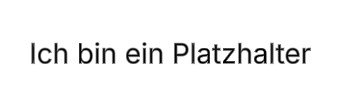
\includegraphics[width=0.3\linewidth]{inhalt/bilder/Platzhalter.jpg}
%     \caption{HTML-Benutzeroberfläche der Wortuhr. Über diese können die Wortuhr ein- und ausgeschaltet, die Helligkeit angepasst und die Farbe der LEDs verändert werden. Weiterhin können aktuelle Statusinformationen der Wortuhr überwacht werden.}
%     \label{fig:Benutzeroberflaeche}
% \end{figure}

Zur Steuerung des Systems wird ein integrierter Webserver implementiert, welcher direkt auf dem Mikrocontroller ausgeführt wird.  
Die Kommunikation erfolgt über HTTP und der Zugriff ist über einen Webbrowser möglich.
Die Benutzeroberfläche ermöglicht das Ein- und Ausschalten der Wortuhr sowie die Anpassung von Helligkeit und Farbwerten.  
Die Verarbeitung der Nutzereingaben erfolgt über URL-Parameter.

\begin{lstlisting}[style=arduino,caption={Verarbeitung der Nutzereingaben ueber URL-Parameter}]
void handleSet() {
  bool changed = false;

  if (server.hasArg("power")) {
    int p = server.arg("power").toInt();
    lampPower = (p != 0);
    changed = true;
  }

  if (server.hasArg("brightness")) {
    int b = server.arg("brightness").toInt();

    if (b < 0) b = 0;
    if (b > 100) b = 100;

    webBrightness = b;
    changed = true;
  }

  if (changed) {
    showHourWord(currentHour);
  }

  server.sendHeader("Location", "/", true);
  server.send(302, "text/plain", "OK");
}
\end{lstlisting}

Zusätzlich wird eine JSON-Schnittstelle bereitgestellt, über welche Statusinformationen für externe Anwendungen ausgelesen werden können.  
Die HTML-Benutzeroberfläche wird dynamisch auf dem ESP32 erzeugt und über den integrierten HTTP-Server bereitgestellt.  
Weitere Funktionen zur Generierung der HTML-Seite, API-Ausgabe und Verarbeitung von Browseranfragen befinden sich im vollständigen Programmcode in Anhang~\ref{apx:1}.  

Die Benutzeroberfläche kann als Web-App direkt zum Homebildschirm eines mobilen Endgeräts hinzugefügt werden.  
Dadurch lässt sich die Steuerung der Wortuhr ähnlich wie eine native Smartphone-Anwendung bedienen (vgl. Abbildung~\ref{fig:APIHomebildschirm}).

\begin{figure}[H]
    \centering
    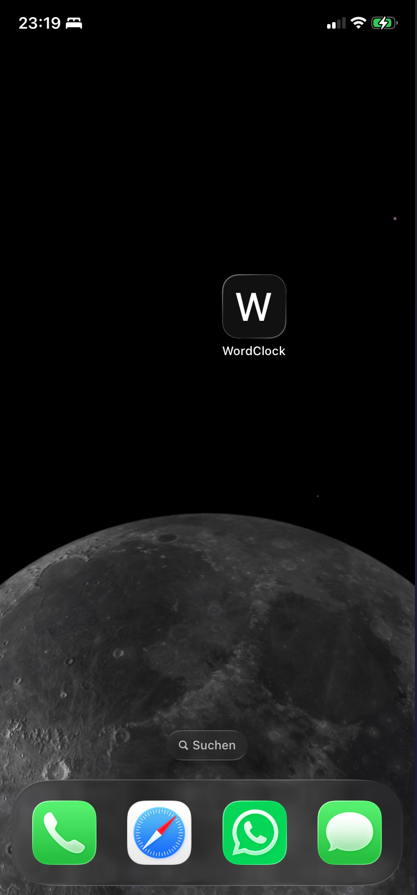
\includegraphics[width=0.4\linewidth]{inhalt/bilder/APIHomebildschirm.png}
    \caption{Die HTML-Benutzeroberfläche kann als Web-App zum Homebildschirm hinzugefügt werden und ermöglicht dadurch einen schnellen Zugriff auf die Steuerung der Wortuhr.}
    \label{fig:APIHomebildschirm}
\end{figure}

Nach dem Öffnen der Benutzeroberfläche werden zunächst die aktuellen Statusinformationen der Wortuhr angezeigt.  
Hierzu zählen unter anderem Uhrzeit, Wetterdaten, Helligkeit, Farbwerte sowie Sensorinformationen (vgl. Abbildung~\ref{fig:APIParameteruebersicht}).

\begin{figure}[H]
    \centering
    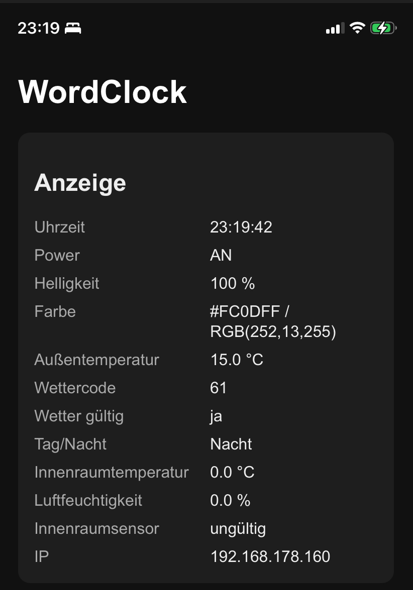
\includegraphics[width=0.4\linewidth]{inhalt/bilder/APIParameterübersicht.png}
    \caption{Übersicht der aktuellen Systemparameter und Statusinformationen innerhalb der HTML-Benutzeroberfläche.}
    \label{fig:APIParameteruebersicht}
\end{figure}

Im unteren Bereich der Benutzeroberfläche befinden sich die Bedienelemente.  
Über diese kann die Wortuhr ein- und ausgeschaltet sowie eine manuelle Aktualisierung der Wetterdaten ausgelöst werden (vgl. Abbildung~\ref{fig:APIEinAus}).

\begin{figure}[H]
    \centering
    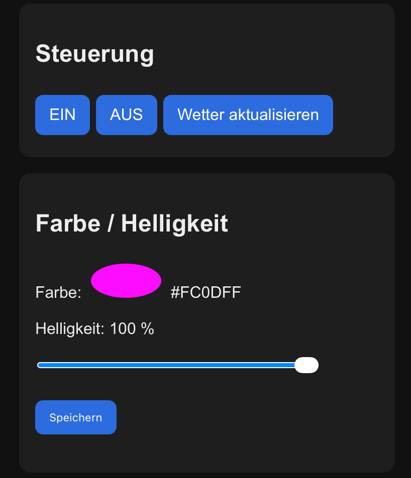
\includegraphics[width=0.4\linewidth]{inhalt/bilder/APIEINAUSFARBE.png}
    \caption{Bedienelemente der HTML-Benutzeroberfläche zur Steuerung der Wortuhr und zur Aktualisierung der Wetterinformationen.}
    \label{fig:APIEinAus}
\end{figure}

Zusätzlich können Helligkeit und Farbe der LED-Beleuchtung angepasst werden.  
Die Helligkeit wird über einen Slider eingestellt, während die Farbe über einen integrierten Farbwähler ausgewählt werden kann (vgl. Abbildung~\ref{fig:APIFarbe}).

\begin{figure}[H]
    \centering
    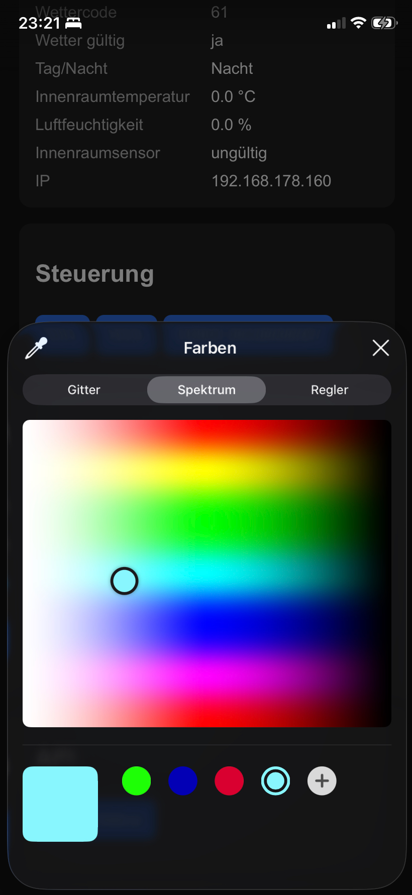
\includegraphics[width=0.4\linewidth]{inhalt/bilder/APIFarbe.png}
    \caption{Einstellmöglichkeiten für Helligkeit und Farbe der LED-Beleuchtung innerhalb der mobilen Benutzeroberfläche.}
    \label{fig:APIFarbe}
\end{figure}

% Zusätzlich wird eine JSON-Schnittstelle bereitgestellt, über welche Statusinformationen für externe Anwendungen ausgelesen werden können.  
% Die HTML-Benutzeroberfläche wird dynamisch auf dem ESP32 erzeugt und über den integrierten HTTP-Server bereitgestellt.
% Weitere Funktionen zur Generierung der HTML-Seite, API-Ausgabe und Verarbeitung von Browseranfragen befinden sich im vollständigen Programmcode in Anhang~\ref{apx:1}.
% Die Benutzeroberfläche und verwendung dieser ist in Abbildung~\ref{fig:Benutzeroberflaeche} dargestellt.

% \begin{figure}[H]
%     \centering
%     \begin{subfigure}[t]{0.3\textwidth}
%         \centering
%         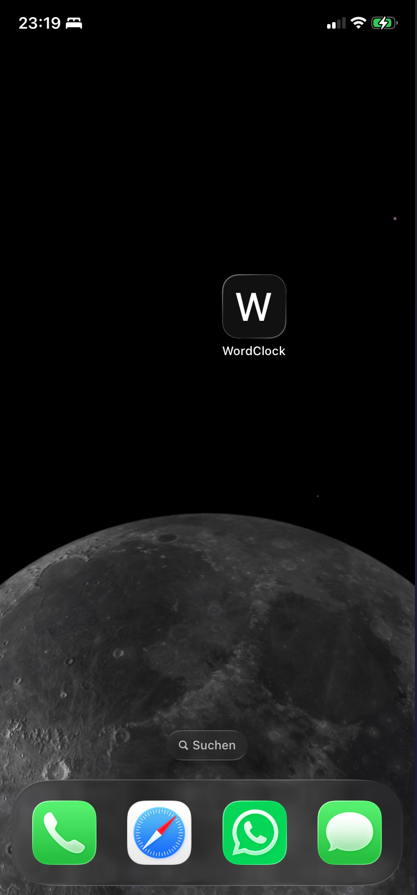
\includegraphics[width=\linewidth]{inhalt/bilder/APIHomebildschirm.png}
%         \caption{Die HTML-Benutzeroberfläche kann als Web App zum Homebildschirm hinzugefügt werden wodurch sich die API wie eine App öffnen und bedienen lässt.}
%         \label{fig:sub_a}
%     \end{subfigure}
%     \hfill
%     \begin{subfigure}[t]{0.4\textwidth}
%         \centering
%         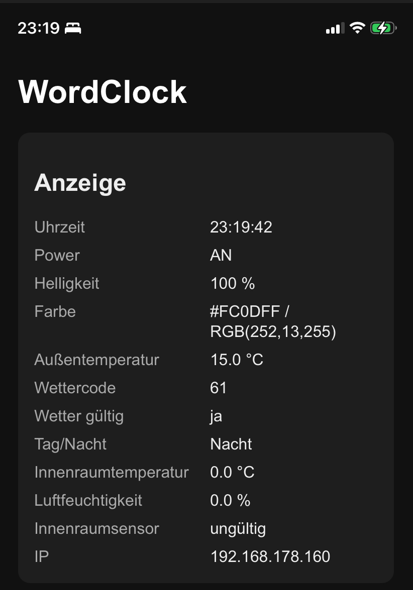
\includegraphics[width=\linewidth]{inhalt/bilder/APIParameterübersicht.png}
%         \caption{Beim öffnen der API sieht man im oberen Teil zunächst eine Übersicht aller Variablen und deren aktuelle Werte.}
%         \label{fig:sub_b}
%     \end{subfigure}
%     \vspace{0.8em}
%     \begin{subfigure}[t]{0.4\textwidth}
%         \centering
%         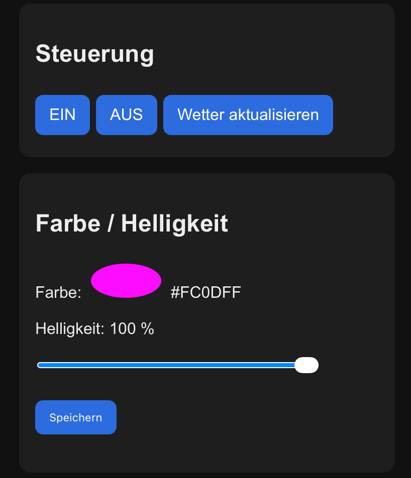
\includegraphics[width=\linewidth]{inhalt/bilder/APIEINAUSFARBE.png}
%         \caption{Im unteren Teil sieht man die Bedienflächen um die Wortuhr ein- und auszuschalten, sowie eine aktualisierung der Wetterinformationen zu initialisieren. Darunter befindet sich die Schaltfläche für die Farb- und Helligkeitssteuerung.}
%         \label{fig:sub_c}
%     \end{subfigure}
%     \hfill
%     \begin{subfigure}[t]{0.4\textwidth}
%         \centering
%         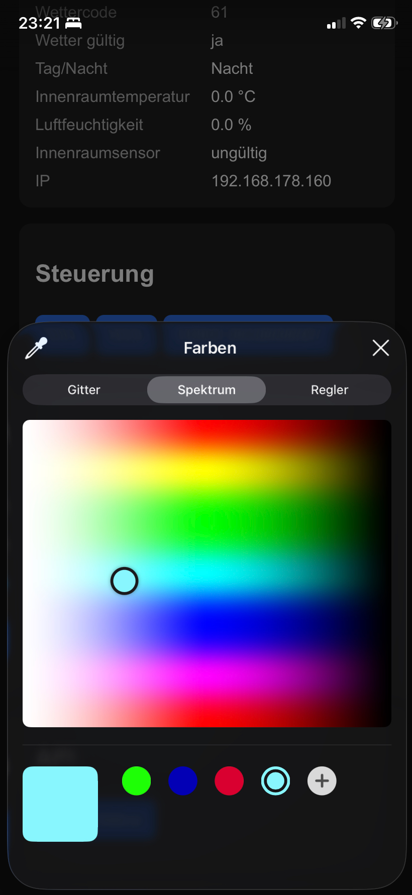
\includegraphics[width=\linewidth]{inhalt/bilder/APIFarbe.png}
%         \caption{Die Helligkeit lässt sich über den Slider regeln. Für die Farbeinstellung kommt man in dieses Fenster und kann die gewünschte Farbe auswählen. Zusätzlich kann man sich im unteren Teil Favoriten abspeichern.}
%         \label{fig:sub_d}
%     \end{subfigure}
%     \caption{HTML-Benutzeroberfläche der Wortuhr. Über diese können die Wortuhr ein- und ausgeschaltet, die Helligkeit angepasst und die Farbe der LEDs verändert werden. Zusätzlich lassen sich aktuelle Statusinformationen überwachen.}
%     \label{fig:Benutzeroberflaeche}
% \end{figure}